\documentclass[11pt]{article}

% ── Packages ────────────────────────────────────────────────
\usepackage[margin=1in]{geometry}
\usepackage{amsmath, amssymb, amsthm}
\usepackage{booktabs}
\usepackage{graphicx}
\usepackage{hyperref}
\usepackage{natbib}
\usepackage{setspace}
\usepackage{microtype}
\usepackage{enumitem}
\usepackage{caption}
\usepackage{subcaption}
\usepackage{xcolor}
\usepackage{float}
% code packages
\usepackage{listings}
\usepackage{inconsolata}
\lstset{basicstyle=\ttfamily\footnotesize,breaklines=true}
\usepackage{csvsimple}
\usepackage{booktabs}

% ── Hyperref setup ──────────────────────────────────────────
\hypersetup{
    colorlinks = true,
    linkcolor  = black,
    citecolor  = black,
    urlcolor   = blue
}

% ── Theorem environments ────────────────────────────────────
\newtheorem{theorem}{Theorem}
\newtheorem{proposition}{Proposition}
\newtheorem{lemma}{Lemma}
\newtheorem{corollary}{Corollary}
\theoremstyle{definition}
\newtheorem{definition}{Definition}
\newtheorem{assumption}{Assumption}
\theoremstyle{remark}
\newtheorem{remark}{Remark}

% ── Spacing ─────────────────────────────────────────────────
\onehalfspacing

% ── Title block ─────────────────────────────────────────────
\title{Love of Variety: September 22nd Update}
\author{Tate Mason}
\date{\today}

% ============================================================
\begin{document}
\maketitle
\thispagestyle{empty}

\section{Overview}

After submission of my first draft of this project, I have updated the time frame from 2014 alone to 2022-2024. This was done for a couple of reasons. First, I wanted more households in my sample. The filter to single agent households cuts a lot of potential observations, so increasing the time horizon could be a good way to remedy this. Secondly, and more importantly, Nielsen updated their data to include more product characteristics in 2021. This allows me to include characteristics like fat, sugar, and protein content of the yogurt as well as overall calorie count. When merging this with flavors, I can get a better idea of the dimensions along which consumers switch.

I have also added markets. The complete list of markets are now Atlanta, Chicago, Denver, Des Moines, Houston, Philadelphia, Phoenix, and San Diego. This geographic spread is nice for my IV approach as I now have representation across most of the country. For my IV to correct endogeneity in prices, I plan to try a few specifications. One is cold brew prices since all of the major yogurt manufacturers or their parent company produce cold brew. Since cold brew would also be subject to any supply shocks along distribution lines while not using inputs related to yogurt, I think it would be an appropriate instrument. Of course, I am happy to discuss this further. The other IV specifications include price of coffee creamer and cost of fruit.

Following Eli and Peter's advice, I will be modeling each trips yogurt purchases within a given week as stocking up for that week. That is, if $HH_i$ buys 3 cups of yogurt in a trip, they chose the outside option four times since that is four days without yogurt. If they go multiple times, say, $HH_i$ buys 3 cups during trip $t$ and 2 more during trip $t+1$, they have taken the outside option a combined 9 times. I think there are ways to iterate on this, but for a starting point I plan to keep it simple and build it up. Happy to discuss further from here.

\section{Summary Statistics}

Summary stats are not substantially different. A key difference is an increase to 5,397 total households in the sample and 3,378 yogurt buying households. Each household has an average of 84 unique trips with about 11 yogurt purchases per trip. Mean income is between 40-45,000. Each trip, 90.5\% of households take the outside option. And about 28\% purchase with a coupon. Average age is around 55 years old. When we look at flavor switching behavior, households buy a flavor for about 28 consecutive periods before switching. A household does switch just under 5 times in their 8 weeks of observations. 69\% of households are ever-switchers and 30.6\% of switchers use a coupon for that purchase.

These stats are relatively similar, though trip numbers are inflated and thus consecutive buys are as well. The sample is also much older for men, though a similar range for women. I will continue to investigate interesting patterns and get switching dynamics around the other characteristics mentioned. Lastly, I will look into the trip counts to ensure there is no inflation. While my code is correct, this result just feels high.

\section{Figures}

Now, we can look at our trusty heat map, with some actual change this time. Now, we see consumer of other flavors are the stickiest group. This is likely a byproduct of other having so many flavors wrapped up in it. Would love some advice on how to tackle this, if even necessary. For those switching from berry to other flavors, they stay on other for 7.7 trips. For plain to other it is 7.9 trips. From berry to plain is 7 trips, other to berry is 5.7, other to plain is 5.1, and plain to berry is 5. This is quite different from last time, with plain being far and away the flavor households would stay on. Further, this trip inflation also bleeds into here. Again, I will continue to investigate this. 

\section{Supply}

Eli and Peter also suggested starting on a toy model of the supply side so I could find their optimal advertising levels. I took a first pass at it and will describe below.

Assume there are two types of individuals: high-switchers $\gamma_h$ and low-switchers $\gamma_{\ell}$. Each type is advertised to at one of two levels, $a_h \ \text{or} \ a_{\ell}$. Further, each type has a probability of advertising working on them, $\theta_i$ for $i = \{\ell,h\}$. The cost of advertising takes the following form:

\begin{align*}
  C(a_{\ell}, a_h) = \frac{c}{2}(a_{\ell}^2 + a_h^2)
\end{align*}

Where $c$ is a flat cost which is evenly split across both types of advertising. The quantity purchased looks as such:

\begin{equation*}
q_i(a_i)
=
\theta_i a_i-\frac{(\gamma_i a_i)^2}{2}.
\end{equation*}

Where quantity purchased is a function of advertising. The first term represents how the probability of the ad working scaled by advertising intensity while the second is how impactful advertising is on that type. Finally, the firm's profit function:

\begin{equation*}
\max_{a_\ell,a_h} \;
\pi(a_\ell,a_h)
=
\sum_{i\in\{\ell,h\}}
m(1+\beta\gamma_i)
\left(
\theta_i a_i-\frac{(\gamma_i a_i)^2}{2}
\right)
-\frac{c}{2}(a_\ell^2+a_h^2).
\end{equation*}

We sum over both types where the first time is two-period profit margin $m(1+\beta\gaamma_i)$, derived from $m(1+\beta\gamma_i) = m + \beta\gamma_i m$, times the quantity purchased $q_i(a_i)$. The second term just subtracts off costs $C(a_{\ell}, a_h)$. Now, we can differentiate with respect to $a_i$ and yield the following:

\begin{align*}
\frac{\partial \pi}{\partial a_i}
&= m(1+\beta\gamma_i)(\theta_i-\gamma_i^2a_i)-ca_i=0, \\[4pt]
a_i^*
&= \frac{\theta_i m(1+\beta\gamma_i)}
{c+\gamma_i^2m(1+\beta\gamma_i)}.
\end{align*}

Thus, the optimal advertising level for either type is their probability times the profit margin divided by the cost added to the type-affected profit margin. That is, the margin may differ depending on which type you produce for. They are symmetric since all but $a_i$ is an assigned type from the beginning of the model. Again, this is just a first pass so I am happy to add or omit anything. Just let me know.

\section{Concluding and Next Steps}

I am struggling with the data still. The retail and panel merge is taking days due to some weird key mismatches. I think I am in the home stretch, but still WIP. Once that is done, I will begin on reworking my estimation code to include more characteristics, incorporate the new timing, and incorporate random coefficients. Let me know any questions, comments, or concerns and always happy to meet to discuss.


% Add to preamble:
\usepackage{booktabs}

\begin{table}[htbp]
    \centering
    \caption{Full Sample Summary Statistics}
    \label{tab:summary_stats}
    \begin{tabular}{lr}
        \toprule
        Statistic & Value \\
        \midrule
        Number of households in full sample
            & 5,397 \\
        Number of yogurt-purchasing households
            & 3,378 \\
        Mean number of trips per household
            & 84.47 \\
        Mean number of yogurt purchases per trip (purchasers)
            & 10.68 \\
        Mean household income
            & \$40,000-45,000 \\
        Percent taking outside option each trip
            & 90.54\% \\
        Percent purchasing with coupon
            & 27.87\% \\
        Average age (overall)
            & 55 \\
        Average age (male)
            & 55 \\
        Average age (female)
            & 55 \\
        \bottomrule
    \end{tabular}
\end{table}

\begin{figure}[htbp]
  \centering
  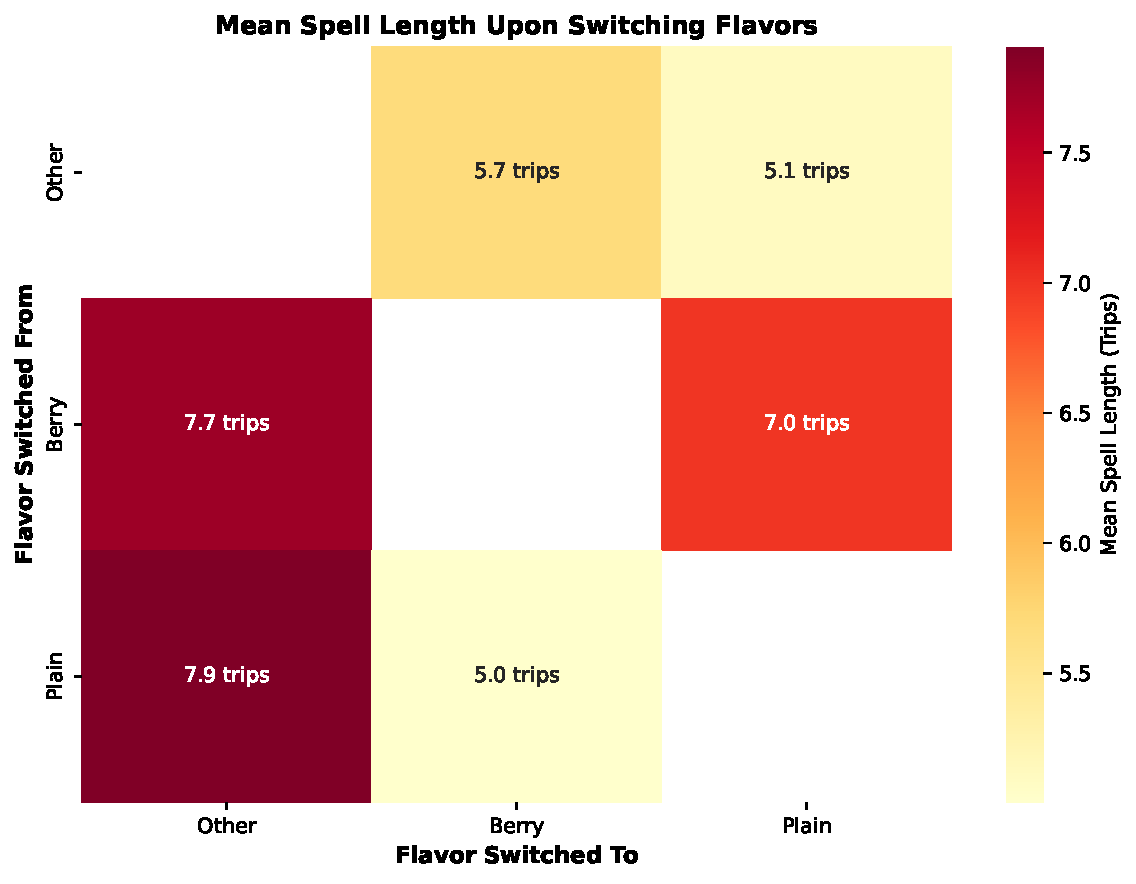
\includegraphics[width=\textwidth]{../../../Output/Plots/3_flav_heatmap.pdf}
  \caption{}
  \label{fig:heatmap}
\end{figure}

\end{document}


